%
% File eacl2014.tex
%
% Contact g.bouma@rug.nl yannick.parmentier@univ-orleans.fr
%
% Based on the instruction file for ACL 2013 
% which in turns was based on the instruction files for previous 
% ACL and EACL conferences

%% Based on the instruction file for EACL 2006 by Eneko Agirre and Sergi Balari
%% and that of ACL 2008 by Joakim Nivre and Noah Smith

%\documentclass[11pt,letterpaper]{article}
%\usepackage{naaclhlt2015}
%\usepackage{times}
%\usepackage{latexsym}

%%\documentclass[11pt]{article}
%%\usepackage{acl2014}
%%\usepackage{times}
%%\usepackage{latexsym}
%\usepackage{url}
%\usepackage{graphicx}
%\usepackage{color}
%\usepackage{comment}
%\usepackage{times}
%\usepackage{amsmath,amsthm,amssymb}
%\usepackage{multirow}
%\usepackage{url}
%\usepackage{verbatim}
%\usepackage{caption}
%\usepackage{subcaption}
%\usepackage{fixltx2e}
%%\usepackage[options]{natbib}
%\usepackage{float}
%%\usepackage{covington}
%\usepackage{supertabular,booktabs}
%%\usepackage[ruled,vlined,linesnumbered]{algorithm2e}
%\usepackage{enumerate}
%\usepackage{longtable}
%\usepackage{afterpage}
%\usepackage{array}
%%\usepackage{setspace}
%\captionsetup{font={footnotesize}}


%\special{papersize=210mm,297mm} % to avoid having to use "-t a4" with dvips 
%\setlength\titlebox{5cm}  % You can expand the title box if you really have to

%\newcommand{\svmr}{{SVM$^{rank}$}}
%\newcommand{\code}[1]{{\tt {\small #1}}}
%\newcommand{\qn}{{{\bf Q}$^\textbf{{\small N}}$}}
%\newcommand{\ssa}{{{\scriptsize $^{*}$}}}
%\newcommand{\todo}[1]{\textcolor{red}{#1}}

%\title{Spinning Straw into Gold: Using Free Text to Train Monolingual Alignment Models for Non-factoid Question Answering}



%\begin{abstract}
%Monolingual alignment models have been shown to boost the performance of question answering systems by "bridging the lexical chasm" between questions and answers.
%%and associating question words like {\em breakfast} with answer words like {\em pancakes} or {\em cereal}.  %Unfortunately these models have been historically challenging to generate, requiring large and expensive corpora of aligned QA pairs to train.  
%The main limitation of these approaches is that they require semistructured training data in the form of question-answer pairs, which is difficult to obtain in specialized domains or low-resource languages.
%%While these models currently require semistructured training data in the form of question-answer pairs, 
%We propose two inexpensive methods for training alignment models solely using free text, by generating artificial question-answer pairs from discourse structures. Our approach is driven by two representations of discourse: a shallow sequential representation, and a deep one based on Rhetorical Structure Theory. 
%We evaluate the proposed model on two corpora from different genres and domains: one from Yahoo! Answers and one from the biology domain, and two types of non-factoid questions: manner and reason. We show that these alignment models trained directly from discourse structures imposed on free text
%improve performance considerably over an information retrieval baseline and a neural network language model trained on the same data.
%%
%%imposing discourse structure on free text allows high-quality alignment models to be inexpensively trained, and that these models can improve performance up to 49\% (relative) over strong information retrieval and neural network language model baselines. 
%
%\end{abstract}

\chapter{NAACL2015 - ALIGNMENT\label{chapter:naacl2015}}



\section{Introduction}
\vspace{-2mm}

 Question Answering (QA) is a challenging task that draws upon many aspects of NLP.  Unlike search or information retrieval, answers infrequently contain lexical overlap with the question (e.g. {\em What should we eat for breakfast? -- Zoe's Diner has good pancakes}), and require QA models to draw upon more complex methods to bridge this "lexical chasm" \cite{Berger:00}.  These methods range from robust shallow models based on lexical semantics, to deeper, explainably-correct, but much more brittle inference methods based on first order logic.  

Berger et al.~\citeyear{Berger:00} proposed that this "lexical chasm" might be partially bridged by repurposing statistical machine translation (SMT) models for QA. Instead of translating text from one language to another, these monolingual alignment models learn to translate from question to answer\footnote{In practice, alignment for QA is often done from answer to question, as answers tend to be longer and provide more opportunity for association~\cite{Surdeanu:11}.}, learning common associations from question terms such as {\em eat} or {\em breakfast} to answer terms like {\em kitchen, pancakes, or cereal}.

While monolingual alignment models have enjoyed a good deal of recent success in QA (see related work), they have expensive training data requirements,  
requiring a large set of aligned in-domain question-answer pairs for training.
% ms: this footnote dilutes the message: too specific for this discussion.
%\footnote{We have empirically observed that alignment models tend to generalize better between training and test folds when the alignment model is trained on its own fold, further increasing the number of high-quality QA pairs required.}.  
%In most domains these pairs are expensive to generate, and one of the current methodological challenges in QA is locating or building high-quality QA pairs for training and testing. Even large open-domain international evaluations and workshops such as the Text REtrieval Conference (TREC)\footnote{\url{http://trec.nist.gov}} and the Cross Language Evaluation Forum (CLEF),\footnote{\url{http://www.clef-initiative.eu}} are often limited to sets of a few hundred factoid questions, many of which are highly related.  As a result, for open domain QA one often makes use of Community Question Answering (CQA) data from websites such as Yahoo! Answers or Stack Overflow, which offer tens of thousands of questions, but of highly variable quality.  
For low-resource languages or specialized domains like science or biology, often the only option is to enlist a domain expert to generate gold QA pairs --  a process that is both expensive and time consuming.  All of this means that only in rare cases are we accorded the luxury of having enough high-quality QA pairs to properly train an alignment model, and so these models are often underutilized or left struggling for resources. 

Making use of recent advancements in discourse parsing \cite{feng12}, here we address this issue, and investigate whether alignment models for QA can be trained from artificial question-answer pairs generated from discourse structures imposed on free text.
% by imposing structure on inexpensive free text resources instead of using QA pairs.  
We evaluate our methods on two corpora, generating alignment models for an open-domain  community QA task using Gigaword\footnote{LDC catalog number LDC2012T21}, and for a biology-domain QA task using a biology textbook. 

The contributions of this work are:
\begin{enumerate}
\vspace{-3mm}
\item We demonstrate that by exploiting the discourse structure of free text, monolingual alignment models can be trained to surpass the performance of models built from expensive in-domain question-answer pairs. 
\vspace{-3mm}
\item We compare two methods of discourse parsing: a simple sequential model, and a deep model based on Rhetorical Structure Theory (RST)~\cite{mann88}.  We show that the RST-based method captures within and across-sentence alignments and performs better than the sequential model, but the sequential model is an acceptable approximation when a discourse parser is not available.  
\vspace{-3mm}
\item We evaluate the proposed methods on two corpora, including a low-resource domain where training data is expensive (biology).
\vspace{-3mm}
\item We experimentally demonstrate that monolingual alignment models trained using our method considerably outperform state-of-the-art neural network language models in low resource domains.
\end{enumerate}










%the task of question answering (QA) has received considerable attention. However, most of this effort has focused on factoid questions rather than more complex non-factoid (NF) questions, such as manner, reason, or causation questions. Moreover, the vast majority of QA models explore only 
%%similarity models based on 
%local linguistic structures, such as syntactic dependencies or semantic role frames, which are generally restricted to individual sentences. This is problematic for NF QA, where questions are answered 
% not by atomic facts, but 
%by larger cross-sentence conceptual structures that convey the desired answers. Thus, to answer NF questions, one needs a model of what these answer structures look like.
%
%Driven by this observation, our main hypothesis is that the discourse structure of NF answers provides complementary information to state-of-the-art QA models that measure the similarity (either lexical and/or semantic) between question and answer. 
%We propose a novel answer reranking (AR) model that combines lexical semantics (LS) with discourse information, driven by two representations of discourse: a shallow representation centered around discourse markers and surface text information, and a deep one based on the Rhetorical Structure Theory (RST) discourse framework~\cite{mann88}.
%To the best of our knowledge, this work is the first to systematically explore within- and cross-sentence structured discourse features for NF AR. The contributions of this work are:
%\begin{enumerate}
%\vspace{-3mm}
%\item We demonstrate that modeling discourse is greatly beneficial for NF AR for two types of NF questions, manner ({\em ``how"}) and reason ({\em ``why"}), across two large datasets from different genres and domains -- one from the community question-answering (CQA) site of Yahoo! Answers\footnote{\url{http://answers.yahoo.com}}, and one from a biology textbook.  
%%Our results show statistically significant improvements of over 20\%, up to 37\% (relative) on precision at 1 (P@1) when discourse is considered. Crucially, these improvements hold even on top of state-of-the-art LS models~\cite{yih13}.
%Our results show statistically significant improvements of up to 24\% on top of state-of-the-art LS models~\cite{yih13}.
%\vspace{-3mm}
%\item We demonstrate that both shallow and deep discourse representations are useful, and, in general, their combination performs best.
%\vspace{-3mm}
%\item We show that discourse-based QA models using inter-sentence features considerably outperform single-sentence models when answers span multiple sentences.
%\vspace{-3mm}
%\item We demonstrate good domain transfer performance between these corpora, suggesting that answer discourse structures are largely independent of domain, and thus broadly applicable to NF QA. 
%\end{enumerate}
%


\section{Related Work}
\label{sec:related work}
%\vspace{-2mm}


Lexical semantic models have shown promise in bridging Berger et al.'s \citeyear{Berger:00} "lexical chasm."  In general, these models can be classified into alignment models \cite{echihabi2003noisy,Soricut:06,Riezler:etal:2007,Surdeanu:11,yao2013} which require structured training data, and language models ~\cite{jansen14,sultan-etal:2014:TACL,yih13}, which operate over free text.  Here, we close this gap in resource availability by developing a method to train an alignment model over free text by making use of discourse structures. 

  
  
%  are focusing here on alignment models, which have shown great promise but also have previously been limited by availability of training data.  We address the need for larger amounts of high quality aligned pairs by investigating methods of imposing structure over free text.... Rhetorical Structure Theory (RST) discourse framework ~\cite{mann88}.

Discourse has been previously applied to QA to help identify answer candidates that contain explanatory text (e.g. Verberne et al. \citeyear{Verberne:2007}).
%conducted an initial analysis of using discourse features derived from Rhetorical Structure Theory (RST)~\cite{mann88} for answer candidate selection, and concluded that while discourse features appeared useful, automated discourse parsing tools were required to test the idea on a larger scale.  
Jansen et al. \citeyear{jansen14} proposed a reranking model that used both shallow and deep discourse features to identify answer structures in large answer collections across different tasks and genres.  Here we use discourse to impose structure on free text to create inexpensive knowledge resources for monolingual alignment. Our work is conceptually complementary to that of Jansen et al. -- where they explored largely unlexicalized discourse structures to identify explanatory text, we use discourse to learn lexicalized models for semantic similarity.

Our work is conceptually closest to that of Hickl et al. \citeyear{hickl2006recognizing}, who created artificially aligned pairs for textual entailment.  Taking advantage of the structure of news articles, wherein the first sentence tends to provide a broad summary of the article's contents, Hickl et al. aligned the first sentence of each article with its headline.  By making use of automated discourse parsing, here we go further and impose alignment structure over an entire text.


%Here, by imposing alignment structure using RST we are able to make use of an entire text instead of being limited to a single sentence.


%
% Example of alignment models
%
%\begin{table}[t!]
%\begin{center}
%\begin{scriptsize}
%\begin{tabular}{l|p{60mm}}
%Passage	& Bob likes apples, which grow in his orchard.  He uses them for cider.  \\
%\hline
%Sequential & Bob likes apples, which grow in his orchard. $\rightarrow$ He uses them for cider. \\
%\hline
%RST & Bob likes apples, $\rightarrow$ which grow in his orchard. \\
% & Bob likes apples, which grow in his orchard. $\rightarrow$ He uses them for cider. \\
%
%
%\end{tabular}
%\end{scriptsize}
%%\vspace{-4mm}
%\caption{{\footnotesize \label{font-table} 
%An example of the alignments produced by the two discourse models.  While the sequential model aligns at sentence granularity capturing only intersentence information, the RST model aligns on finer EDU boundaries, capturing both inter/intrasentence alignments.
%}}
%\vspace{-4mm}
%
%\label{tab:examples}
%\end{center}
%\end{table}


\begin{figure}[t!]
\begin{center}
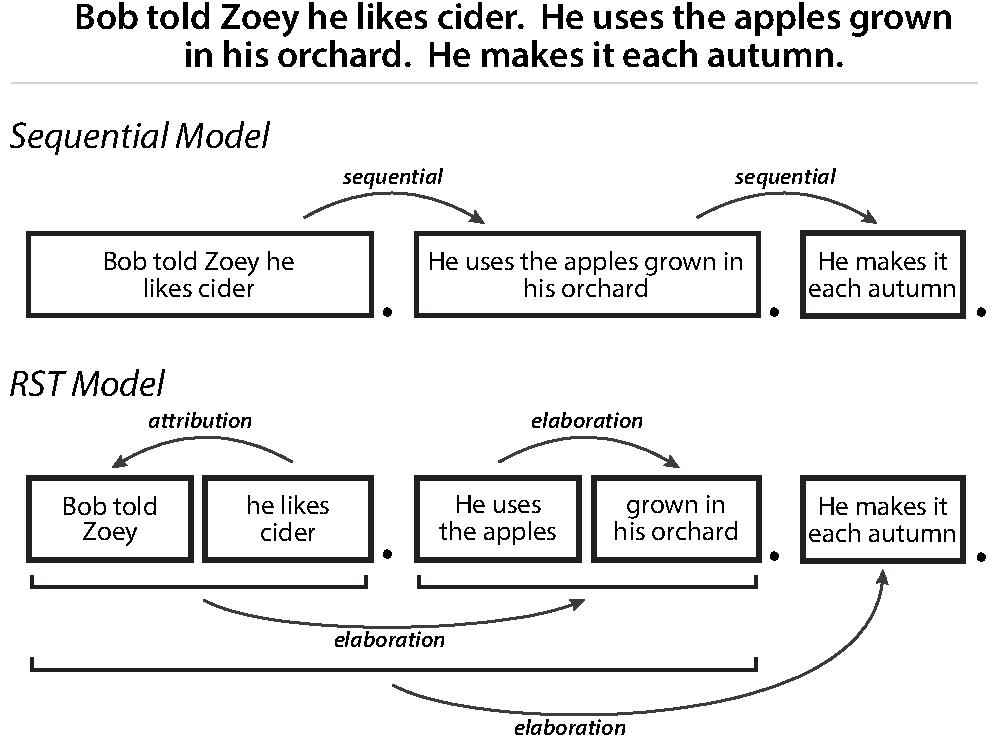
\includegraphics[width=75mm]{rst2a.pdf}
\vspace{-2mm}
\caption{{\small An example of the alignments produced by the two discourse models.  The sequential model aligns pairs of consecutive sentences, capturing intersentence associations such as \emph{cider--apples}, and \emph{orchard--autumn}.  The RST model generates alignment pairs from participants in all (binary) discourse relations, capturing both intrasentence and intersentence alignments, including 
\emph{apples--orchard, cider--apples}, and \emph{cider--autumn}.}}
% ms: I get the point, but there is value in brevity. Plus, maybe we should not use Bob as example :)
%the intersentence alignments above along with intrasentence and multi-sentence alignments, including \emph{Bob--cider, apples--orchard}, and \emph{cider--autumn}.}}
\vspace{-5mm}
\label{fig:examples}
\end{center}
\end{figure}

\vspace{-1mm}
\section{Approach}
\label{sec:approach}
\vspace{-1mm}

A written text is not simply a collection of sentences, but rather a flowing narrative where sentences and sentence elements depend on each other for meaning -- a concept known as cohesion~\cite{halliday2014cohesion}.  
%We make use of this to generate artificial alignment pairs using discourse.  
Here we examine two methods for generating alignment training data from free text that make use of cohesion: a shallow method that uses only intersentence structures, and a deep method that uses both intrasentence and intersentence structures.
We additionally attempt to separate the contribution of discourse from that of alignment in general by comparing these models against a baseline alignment model which aligns sentences at random.

The first model, the sequential discourse model (SEQ), considers that each sentence continues the narrative  of the previous one, and creates artificial question-answer pairs from all pairs of consecutive sentences.
% ms: no space
%This is similar to a right-attachment baseline in dependency parsing, 
%but operating at sentence granularity rather than word.
Thus, this model takes advantage of intersentence cohesion by aligning the content words\footnote{In pilot experiments, we found that aligning only nouns, verbs, adjectives, and adverbs yielded higher performance.} in each sentence with the content words in the following sentence.  For example, in the passage in Figure \ref{fig:examples}, this model would associate \emph{cider} in the first sentence with \emph{apples} and \emph{orchard} in the second sentence.

The second model uses RST to capture discourse cohesion both within and across sentence boundaries.  
We extracted RST discourse structures using an in-house parser~\cite{Surdeanu:15}, which follows the architecture introduced by Hernault et al.~\citeyear{hernault10} and Feng and Hirst~\citeyear{feng12}.
The parser first segments text into elementary discourse units (EDUs), which may be at sub-sentence granularity, then recursively connects neighboring units with binary discourse relations, such as \emph{Elaboration} or \emph{Contrast}.\footnote{The RST parser performs better on relations which occur more frequently.  We use only relations that occurred at least 1\% of the time.  This amounted to six relations: \emph{elaboration}, \emph{attribution}, \emph{background}, \emph{contrast}, \emph{same-unit}, and \emph{joint}. Using all relations slightly improves performance by 0.3\% P@1.} Our parser differs from previous work with respect to feature generation in that we implement all features that rely on syntax using solely dependency syntax. For example, a crucial feature used by the parser is the dominance relations of Soricut and Marcu~\citeyear{soricut2003}, which capture syntactic dominance between discourse units located in the same sentence. While originally these dominance relations were implemented using constituent syntax, we provide an equivalent implementation that relies on dependency syntax. The main advantage to this approach is speed: the resulting parser performs at least an order of magnitude faster than the parser of Feng and Hirst~\citeyear{feng12}. 

Importantly, we generate artificial alignment pairs from this imposed structure by aligning the governing text (nucleus) with its dependent text (satellite).\footnote{Pilot experiments showed that this direction of alignment performed better than aligning from satellite to nucleus.} 
 Turning again to the example in Figure \ref{fig:examples}, this RST-based model captures additional alignments that are both intrasentence, e.g., \emph{apples--orchard}, and intersentence, e.g., {\em cider--autumn}. 
% intersentence associations of the sequential baseline, in addition it finds an intrasentence association between \emph{apples} and \emph{orchard}. 

%\todo{The random alignment baseline (RND) was created in a similar fashion to the SEQ model, except that the sentences were randomly shuffled first.  In the open domain this shuffling took place within a document, and in the biology domain it was done across the entire of the textbook.}



%----------------------TABLE FORMAT FROM TACL 2015--------

\begin{table*}[h]{}

\begin{scriptsize}

        \centering
        %\resizebox{7.9cm}{!}{
        {
        %\begin{tabular}{p{1cm}|p{3cm}|l}
        \begin{tabular}{p{0.3cm}|p{5cm}|p{8cm}}
        \hspace*{-7pt}  & Feature Group & Feature Descriptions \\
        \toprule
        \multirow{10}{*}
        {\rotatebox[origin=c]{90}{~~~~~~~~~Alignment Models}}
        & { Global Alignment Probability } & p(Q$|$A) according to IBM Model 1 \cite{Brown:93}\\ 
        & {} & {}\\
        & { Jenson-Shannon Distance (JSD) } & {Pairwise JSDs were found between the probability distribution of each content word in the question and those in the answer.  The \textbf{mean, minimum, and maximum JSD values} were used as features. Additionally, composite vectors were formed which represented the entire question and the entire answer and the \textbf{overall JSD} between these two vectors was also included as a feature. See Fried et. al \citeyear{fried2015higher} for additional details.} \\
        \midrule
        \multirow{10}{*}
        {\rotatebox[origin=c]{90}{~~~~~~~~~~~~~~~~~~~~~~~~~~~~~~~~~~RNNLM}}
        & { Cosine Similarity } & {Similar to Jansen et al.~\citeyear{jansen14}, we include as features the {\bf maximum and average pairwise cosine similarity} between question and answer words, as well as the {\bf overall similarity} between the composite question and answer vectors.} \\
        \bottomrule
        \end{tabular}
        }
        %}

\end{scriptsize}

        %\caption{$10$ most important features of each sieve.}
        \caption{Feature descriptions for alignment models and RNNLM baseline.}
        \label{tab:Features}
	\vspace{-6mm}

\end{table*}

%------------------END COPIED TABLE----------------
%space{-1mm}
\section{Models and Features}
\label{sec-naacl2015:models}

We evaluate the contribution of these alignment models using a standard reranking architecture~\cite{jansen14}.
The initial ranking of candidate answers is done using a shallow candidate retrieval (CR) component.\footnote{We use the same cosine similarity between question and answer lemmas as Jansen et al.~\citeyear{jansen14}, weighted using {\em tf.idf}.} % (see Ch. 6, \cite{manning08}).}  
Then, these answers are reranked using a more expressive model that incorporates alignment features alongside the CR score.  As a learning framework we use \svmr , a Support Vector Machine tailored for ranking.\footnote{ \url{http://www.cs.cornell.edu/people/tj/svm_light/svm_rank.html}}
We compare this alignment-based reranking model against one that uses a state-of-the-art recurrent neural network language model (RNNLM)~\cite{mikolov10,mikolov13}, which has been successfully applied to QA previously~\cite{yih13}.


%IBM Model 1 \cite{Brown:93} \todo{GIZA++?} was used to generate the discourse pair matrices described in section \ref{sec-naacl2015:approach} for the alignment models.  Each of these models, along with a Recurrent Neural Network Language Model (RNNLM), was used to rerank candidate answers in a shallow retrieval model which used \svmr , a Support vector Machine tailored for ranking.\footnote{ \url{http://www.cs.cornell.edu/people/tj/svm_light/svm_rank.html}}  
%(See Jansen~\citeyear{jansen14} for detailed architecture.\footnote{We also use his \svmr c of 0.1.}) 

{\flushleft {\bf Alignment Model:}}  The alignment matrices were generated with IBM Model 1 \cite{Brown:93} using GIZA++~\cite{och03}, and the corresponding models were implemented as per Surdeanu et al.~\citeyear{Surdeanu:11} with a global alignment probability. 
%, computing a {\bf global alignment probability}, which is the conditional probability of observing a question given an answer.
% ms: the global prob. operates for the whole Q and A!
%question word given an answer word.
%~\footnote{Within Surdeanu et al.'s~\citeyear{Surdeanu:11} framework, we lightly tuned the smoothing parameter, $\lambda$, to 0.4 and we redistributed the probability mass for each word such that the probability of a word translating to itself was 0.5.}  
We extend this alignment model with features from Fried et al.~\citeyear{fried2015higher} that treat each (source) word's probability distribution (over destination words) in the alignment matrix as a distributed semantic representation, and make use the Jensen-Shannon distance (JSD)\footnote{Jensen-Shannon distance is based on Kullback-Liebler divergence but is a distance metric (finite and symmetric).} between these conditional distributions.  A summary of all these features is shown in Table \ref{tab:Features}.% to derive features representing the {\bf minimum, maximum, and average JSDs} between question and answer words, as well as the {\bf overall JSD} between the composite question and answer distributions. 
%Using the Jensen-Shannon distance (JSD) between conditional distributions, content words in each question were compared with the content words in its answers.  Features were made from the maximum, minimum, and average JSDs.  Composite distributions were also created for the entire question and for each entire candidate answer, and the JSD between these composite distributions was used as a feature. 


{\flushleft {\bf RNNLM:}} We learned word embeddings using the \texttt{word2vec} RNNLM of Mikolov et al. \citeyear{mikolov13}, and include the cosine similarity-based features described in Table \ref{tab:Features}. %Similar to Jansen et al.~\citeyear{jansen14}, we include as features the {\bf maximum and average pairwise cosine similarity} between question and answer words, as well as the {\bf overall similarity} between the composite question and answer vectors. 

%{\flushleft {\bf Hyperparameters}}We used the following very lightly tuned hyperparameters: for \svmr, we used c = 0.1 and for IBM model 1, lambda = 0.4 and self-association of 0.5. \todo{re-write this!! or spread to appropriate places} 

\section{Experiments}
\label{sec-naacl2015:experiments}

%\subsection{Data}
%\label{sec-naacl2015:data}
%\vspace{-2mm}


We tested our approach in two different domains, open-domain and cellular biology. For consistency we use the same corpora as Jansen et al.~\citeyear{jansen14}, which are described briefly here. 

{\flushleft {\bf Yahoo! Answers (YA):}}  Ten thousand open-domain \emph{how} questions were randomly chosen from the Yahoo! Answers\footnote{\url{http://answers.yahoo.com}} community question answering corpus and divided: 50\% for training, 25\% for development, and 25\% for test.  Candidate answers for a given question are selected from the corresponding answers proposed by the community (each question has an average of 9 answers).

{\flushleft {\bf Biology QA (Bio):}} 183 \emph{how} and 193 \emph{why}  questions in the cellular biology domain were hand-crafted by a domain expert, and paired with gold answers in the Campbell's Biology textbook~\cite{Reece:2011}.  Each paragraph in the textbook was considered as a candidate answer.  As there were few questions, five fold cross-validation was used with three folds for training, one for development, and one for test.

%In both set-ups, candidate answers were assigned a candidate retrieval (CR) score based on the lexical similarity of the question to the candidate answer.~\footnote{In the Bio task, the CR also incorporated a similarity between the question and the section containing the candidate answer paragraph.}  That CR score served as both a strong baseline for the models (when used alone) as well as an additional feature to be used alongside the model features described in section \ref{sec-naacl2015:models}.
%\subsection{Sources for Alignment}
%\label{sources}

{\flushleft {\bf Alignment Corpora}}: To train the alignment models we generated alignment pairs from two different resources: Annotated Gigaword \cite{Napoles2012} for YA, and the textbook for Bio.  Each was discourse parsed with the RST discourse parser described in Section~\ref{sec-naacl2015:approach}, which is implemented in the FastNLPProcessor toolkit\footnote{\url{http://github.com/sistanlp/processors}}, using the MaltParser\footnote{\url{http://www.maltparser.org/}} for syntactic analysis.
% and reimplements the discourse model of Feng and Hirst~\citeyear{feng12}, using solely features extracted from dependency syntax.


%To explore the relationship between amount of available training data and performance, after each resource was discourse parsed it was divided into samples of exponentially increasing size.  For AGiga, there were 12 sizes ranging from one document to 10,000 and for the textbook, there were 10 sizes ranging from one subsection up to the entire book (2686 subsections).  Additionally, there were 10 samples for each size to reduce the margin of error. 
%condense this---
%To demonstrate the utility of our approach in generating surrogate training data for limited resource domains, we evaluated the performance of our models with incremental amounts of data.  
%{\flushleft {\bf Annotated gigaword \todo{CITE}(AGiga)}}: After discourse parsing AGiga in its entirety, we randomly selected 10 files.  From each we made 12 samples that exponentially increased in size, from 1 document up to 10,000.~\footnote{The larger samples contained the same documents as the smaller samples from the same file so as to represent consistently growing knowledge.}  
%{\flushleft {\bf Campbells}}:For Bio, Campbell's textbook was divided at the subsection level, discarding any subsection consisting of only a single sentence, for a total of 2686 subsections.  These subsections were shuffled to generate 10 random permutations and 10 samples exponentially increasing in number of subsections were made from each.  

\subsection{Results and Discussion}
\label{sec-naacl2015:results}

\begin{figure}[t!]
\begin{center}
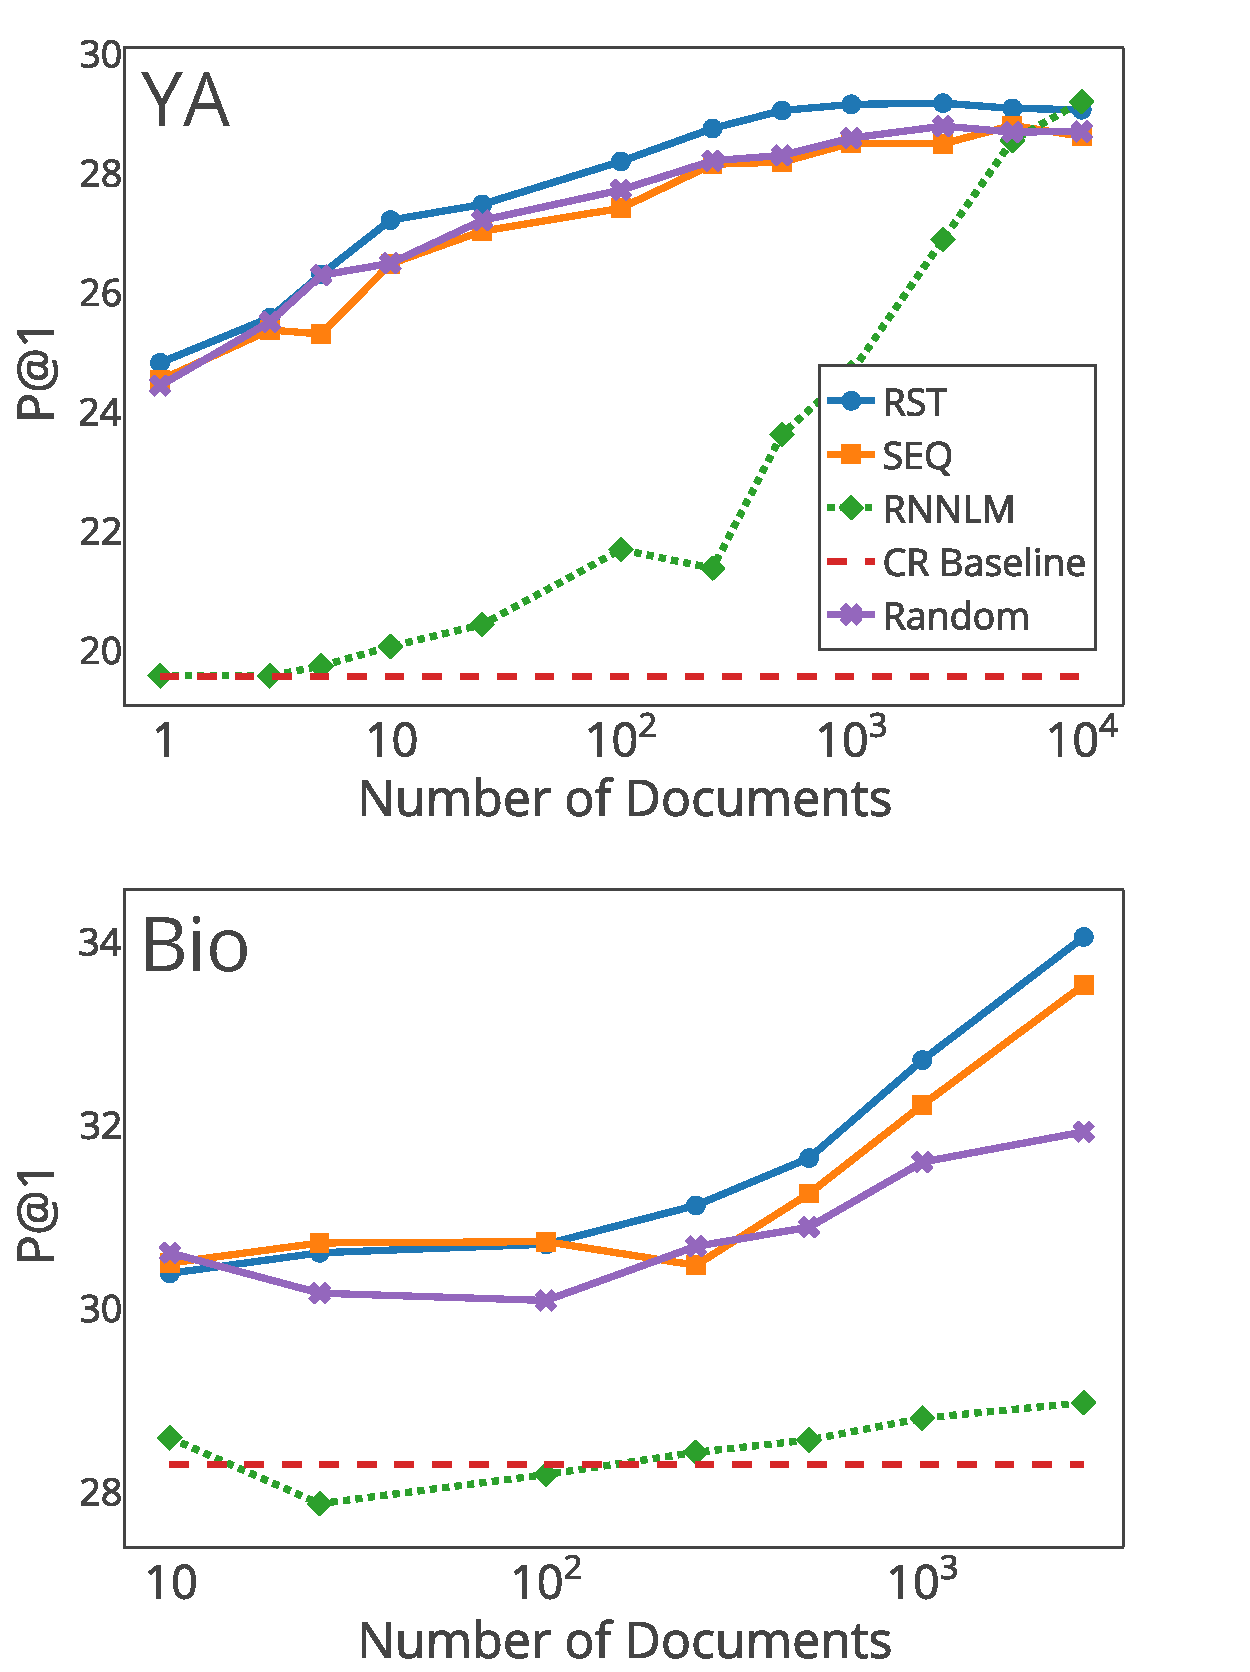
\includegraphics[width=90mm]{mainmatter/naacl2015-alignment/graphs_test2a.pdf}
%\vspace{-4mm}
\caption{{\small Overall performance for the two discourse-based alignment models,
compared against the CR baseline, random baselines, and a RNNLM-based reranker.
%, sequential, and lexical semantic models versus the number of training documents used to construct the models.  
The $x$ axis indicates the number of training documents used to construct all models. 
Each point represents the average of 10 samples of training documents.  }}
%space{-6mm}
\label{fig:performance}
\end{center}
\end{figure}

\begin{comment}
\begin{table}[t!]
\begin{center}
%\begin{scriptsize}
\begin{footnotesize}
\begin{tabular}{llc}
\multicolumn{1}{l}{ } & \multicolumn{1}{l}{ } & \multicolumn{1}{l}{P@1} \\
\multicolumn{1}{l}{ Model/Features } & \multicolumn{1}{l}{P@1} & \multicolumn{1}{l}{Impr.} \\
\cline{2-3}

\hline
\multicolumn{3}{l}{\textit{Yahoo! Answers}} \\ % 185q (sent) ret=1p c=0.1 
\hline
CR Baseline 	& 19.48 	&	  				\\
CR + RST  		& 28.98		& +48.75\% 			\\
CR + SEQ  		& 28.53		& +46.45\% 			\\
CR + RNNLM  		& 29.11		& +49.44\% 			\\
\hline
\multicolumn{3}{l}{\textit{Bio WHY}} \\ % 185q (sent) ret=1p c=0.1 
\hline
CR Baseline 	& 28.24 	&	  				\\
CR + RST  		& 34.00		& +20.38\% 			\\
CR + SEQ  		& 33.47		& +18.53\% 			\\
CR + RNNLM  		& 28.92		& +2.39\% 			\\
\end{tabular}
\end{footnotesize}
\caption{{\small Final performance for the discourse, sequential, and lexical semantic models as compared to the candidate retrieval baseline. For space reasons data for Bio WHY are shown but the pattern is essentially identical for Bio HOW.}}
\label{tab:overall}
\end{center}
\end{table}
\end{comment}
Figure \ref{fig:performance} shows the performance of the discourse models against the number of documents used to train the alignment model.\footnote{For space reasons the graph for Bio \emph{how} is not shown, but the pattern is essentially identical to Bio \emph{why}.}   We used the standard implementation for P@1 ~\cite{manning08} with the adaptations for Bio described in Jansen et al.~\citeyear{jansen14}. We address the following questions.
%, and compare against the CR baseline and RNNLM-based reranker.

\paragraph{How does the performance of the RST and SEQ models compare?}
% and to the baselines?}
Comparing the two principal alignment models, the RST-based model significantly outperforms the SEQ model by about 0.5\% P@1 in both domains (p $<$ 0.001 for Bio and p $<$ 0.01 for YA)\footnote{All reported statistics were performed at the endpoints, i.e., when all training data is used, using bootstrap resampling with 10,000 iterations.}. This shows that deep discourse analysis (as imperfect as it is today) is beneficial. 

\paragraph{How does the performance of the RST model compare to a model trained on in-domain pairs?}

Both the RST and SEQ results for YA are {\em higher} than that of an alignment model trained on explicit in-domain question-answer pairs. Fried et. al \citeyear{fried2015higher} trained an identical alignment model using approximately 65k QA pairs from the YA corpus, and report a performance of 27.24\% P@1, or nearly 2 points lower than our model trained using 10,000 Gigaword documents. This is an encouraging result, which further demonstrates that: (a) discourse analysis can be exploited to generate artificial semi-structured data for alignment, and (b) the sequential model, which also outperforms Fried et. al, can be used as a reasonable proxy for discourse when a parser is not available. 


\paragraph{How does the performance of the RST model compare to previous work?}

Comparing our work to Jansen et al. \citeyear{jansen14}, the most relevant prior work, we notice two trends.
First, our discourse-based alignment models outperform their CR + RNNLM model, which peaks at 26.6\% P@1 for YA and 31.7\% for Bio \emph{why}. While some of this difference can be assigned to implementation differences (e.g., we consider only content words for both alignment and RNNLM, where they used all words), this result again emphasizes the value of our approach.
% Second, while our content-filtered RNNLM outperforms their unfiltered model\footnote{RNNLM performance is slightly less in Bio as we use only the textbook for training.}, when using equal amounts of training data, our alignment model trained using discourse still outperforms the RNNLM until the performance of all models ultimately plateaus in knowledge-rich environments.  
Second, the partially lexicalized discourse structures used by Jansen et. al to identify explanatory text in candidate answers perform better than our approach, which relies solely on lexicalized alignment. However, we expect that our two approaches are complementary, because they address different aspects of the QA task (structure vs. similarity).
%the performance of our alignment models be orthogonal to their discourse models, 
%as we don't explicitly use discourse structures to identify answer candidates in our reranker.

\paragraph{How do the RST and SEQ models compare to the non-alignment baselines?}

%Both the RST and SEQ alignment models \todo{significantly} %considerably 
%outperform the CR and RNNLM baselines, especially for few training documents or domain-specific (Bio) settings.\footnote{The immediate performance boost seen by the alignment models even for 1 training document is explained by the fact the the global alignment probability of Surdeanu et al. (2011) explicitly models word self associations, which complements well the vector space model of the CR baseline.}  

In Bio, both the RST and SEQ alignment models significantly outperform the RNNLM and CR baselines (p $<$ 0.001).  %Additionally, the RST model does significantly better than the SEQ model (p $<$ 0.001).  
In YA, the RST and SEQ models significantly outperform the CR baseline (p $<$ 0.001), and though 
%and the RST model also does significantly better than the RND baseline (p $<$ 0.05) though the SEQ does not (p $>$ 0.1).% as well as the SEQ model (p $<$ 0.01).  
they considerably outperform the the RNNLM baseline for most training document sizes, when all 10,000 documents are used for training, they do not perform  better.  
%Finally, the SEQ model is not significantly better than the RND baseline (p $>$ 0.1).
This shows that alignment models are more robust to little training data, but RNNLMs catch up when considerable data is available.

%RND??
%with both models approaching 34\% P@1 in Bio (or 20\% over the CR baseline), and 29\% P@1 in YA (up to a 49\% relative performance gain over the CR baseline). \textcolor{red}{In YA, when all training documents are used, the performance of the RST model was significantly higher the SEQ model (p $<$ 0.01) as well as all baselines (p $<$ *** for all).  The YA SEQ model performance was not significantly different than that of the RND baseline (p $>$ ***) but was ***.  In Bio...  As the amount of training data in Bio increases, performance gaps of the various models widen.  That is, when enough signal builds up, we can see the increase in efficacy of lexical associations when words go from simply being within the same domain (tRND), to broadly cohesive (SEQ), to finally having a fine-grained discourse connection (RST).}

\paragraph{How does the SEQ model compare to the RND baseline?}
In Bio, the SEQ model significantly outperforms the RND baseline (p $<$ 0.001) but in YA it does not.  This is likely due to differences in the size of the document which was randomized.  In YA, the sentences were randomized within Gigaword articles, which are relatively short (averaging 19 sentences), whereas in Bio the randomization was done at the textbook level.  In practice, as document size decreases, the RND model approaches the SEQ model.


%% Cut for space
%\paragraph{What is the contribution of the individual discourse relations used in generating the alignment pairs?}
%\begin{table}[t!]
%\begin{center}
%\begin{footnotesize}
%\begin{tabular}{llclc}
%\multicolumn{1}{l}{ } & \multicolumn{1}{c}{YA} & \multicolumn{1}{c}{Bio} 		\\
%\multicolumn{1}{l}{ Discourse Relations } & \multicolumn{1}{c}{P@1} & \multicolumn{1}{c}{P@1}		\\
%\cline{2-3}
%\hline
%All  	&  29.23	&	 34.39  \\
%Top 6 (92\% of data)  	& 28.98		& 34.00 	\\
%\end{tabular}
%\end{footnotesize}
%\caption{{Comparison of performance for the discourse model when all discourse relations are used versus when only the top 6 most frequent (\textit{elaboration, attribution, background, contrast, joint, and same-unit}) are used.}}
%\vspace{-6mm}
%\label{tab:ablation}
%\end{center}
%\end{table}
%
%As shown in Table \ref{tab:ablation}, the bulk of the performance comes from using the six most frequent discourse relations (of 18 possible discourse relations).  This is likely due to the fact that these top six relations make up 92\% of all relations in both domains. 



\paragraph{Why does performance plateau in YA and not in Bio?}

With Bio, we exploit all of the limited in-domain training data, and continue to see performance improvements.  With YA, however, performance asymptotes for the alignment models when trained beyond 10,000 documents, or less than 1\% of the Gigaword corpus.  Similarly, when trained over the entirety of Gigaword (two orders of magnitude more data), our RNNLM improves only slightly, peaking at approximately 30.5\% P@1 (or, a little over 1\% P@1 higher).  
We hypothesize that this limitation comes from failing to take context into account. 
%In highly technical domains, such as biology, words like {\em phosphorylation} are non-ambiguous, whereas 
In open domains, alignments such as {\em apple -- \mbox{orchard}} may interfere with those from different contexts, e.g., {\em apple -- computer}, and add noise to the answer selection process.  
%This is empirically supported by the data: in Figure \ref{fig:performance} the steep slope of the Bio corpus shows no signs of decreasing even beyond $10^{3}$ documents, whereas in YA it begins to plateau after $10^{2}$ documents.  This suggests that by incorporating context into alignment models for QA, there is the potential to further capitalize on the remaining training data available. 

%For YA, this is the case until nearly all 10,000 documents are used, at which point the RNNLM finally reaches the performance of the alignment models (RST had 48.75\%, SEQ 46.45\%, and RNNLM 49.44\% P@1 relative over the CR baseline).  
%Not demonstrated with our experimental design, in (hidden for review) the performance of the RNNLM is also shown to plateau around 30\% P@1, even when all of gigaword is used to train the vectors.  
%In the highly technical Bio domain, both the RST and SEQ alignment models far outperform the RNNLM across all sample sizes (20.38\%, 18.53\% and 2.39\% P@1 relative over the CR baseline, respectively).  In both domains, the deep RST model using both intersentence and intrasentence associations outperforms the shallow SEQ model using only intersentence associations.

%In comparison to previous work in Jansen et al \citeyear{jansen14}, for YA our final RNNLM performance is higher due to implementational differences (29.11\% P@1 from 10,000 documents compared to their 26.57\% using all of gigaword).  In Bio, our final RNNLM performance is lower (28.92\% P@1 compared to their 31.73\%) because we trained our RNNLM only on the in-domain textbook, as opposed to the expanded corpus they used.  Both the RST and SEQ models, however, performed better than their RNNLM (34.00\% and 33.47\% P@1 respectively), demonstrating that by using our approach to impose structure for alignment we can attain better results with less data.  Additionally, as we don't explicitly use discourse features, we expect that the performance demonstrated here would be orthogonal to that of their deep and shallow discourse models.

%While performance steadily increases with the size of training data, for both alignment and RNNLM models we asymptote at approximately 30\% P@1 and 10,000 training documents for YA (while we are limited by the available training data for Bio). 







%This is likely due to general alignment model limitations coupled with domain differences between gigaword (a news-domain) and CQA.  As more and more documents are included in training, perhaps the model becomes too far biased towards news to continue to increase performance.  In pilot experiments, we found that using as many as 20 files did not improve performance and in (hidden for review) when all of gigaword is used to train the vectors, the performance of the RNNLM plateaus around the same 30\% P@1. As the data used here is a small fraction of the data available, there is potential for performance increases if more sophisticated techniques, such as topic filtering, are implemented.  

%space{-1mm}
\section{Conclusion}
\label{sec-naacl2015:conclusion}
%space{-2mm}

We propose two inexpensive methods for training alignment models using solely free text, by generating artificial question-answer pairs from discourse structures. 
%Using a RST discourse parser, one method generates both intrasentence and intersentence alignments that can be combined to reach peak performance. For domains where a discourse parser is not available, the second aligns sequential sentences provides a close approximation.  
%Both of these models offer methods for low-resource domains where training data is expensive and/or limited. 
Our experiments indicate that these methods are a viable solution for constructing state-of-the-art QA systems for low-resource domains, or languages where training data is expensive and/or limited.  Since alignment models have shown utility in other tasks (e.g. textual entailment), we hypothesize that these methods for creating inexpensive and highly specialized training data could be useful for tasks other than QA.  

%% Cut for space
%Our generation tool, {\tt Straw2Gold}, is available at: {\small \url{http://nlp.sista.arizona.edu/releases/straw2gold}}.

%Future work should be done to determine the extent of immediate application as well as ways to refine the methods for these other uses.


%By imposing structure over free text,  monolingual alignment can used to achieve large performance gains in non-factoid QA.  When discourse parsing is practical for the domain in question, both intrasentence and intersentence alignments can be combined to reach peak performance, and for domains where this isn't possible, aligning sequential sentences provides a close approximation.  Both of these models offer methods for low-resource domains where training data is expensive and/or limited. 

%---------------------------------------DISCUSSION

%In fact, it is notable how quickly we see performance increases from the alignment models in YA.  In both domains, results are increased due to word self-associations (when the same word appears in both the question and the answer), but with YA there also is a slight correlation between answer length and correctness.  The magnitude of the performance increase due to these factors is essentially shown in the results for the smallest sample size, as one document doesn't contain enough data to provide a real alignment contribution.  
%Taking this into account, the scores still increase quite rapidly for YA.  It could be the case that associations between high frequency verbs drive much of this performance.  If so, then perhaps for the more technical Bio domain, more world-knowledge (encoded in nouns and other parts of speech) is needed,  explaining why we don't see the same immediate performance gain.  To test this, matrices could be made with only verbs, only nouns, or other combinations to determine if one type of association is driving much of the performance and how the domains compare in this respect. 

%After a rapid increase, the performance in YA quickly levels off relative to the amount of input for training.~\footnote{Only a fraction of 1 file is used to achieve the maximal performance for the alignment models.  In pilot experiments, including as many as 20 files did not improve performance. }  This may be a result of a decrease in the signal to noise ratio.  Unlike YA, gigaword is within the news domain.  As more and mode documents are added to training, perhaps the model becomes too far biased towards news to continue to increase performance.  If more sophisticated techniques are implemented, such as topic filtering, potentially the performance in this domain could be even higher.  We don't see the same plateau effect with Bio that we do with YA.  Likely this is due to the fact that the in-domain texbook for Bio was much smaller than gigaword.  

%\todo{strong close}
%---------------------------------------OLD
%when all 10,000 documents are used for training, the models have similar performance.  The asymptotic behavior of the RST and SEQ models is rendered in Figure \ref{fig:performance} and in (hidden for review) the RNNLM is also shown to plateau around 30\% P@1 even when all of gigaword is used to train the vectors.~\footnote{Only a fraction of one file is used to achieve this performance plateau for the alignment models.  In pilot experiments we found that including up to 20 files does not improve performance though it does drastically affect runtime.}.  When fewer documents are used, however, the gap in performance is substantial.  
%Additionally, though not demonstrated with our experimental design, rather than surpass the alignment model performance the RNNLM has been shown to plateau around 30\% P@1 even when all of gigaword is used to train the vectors (hidden for review).    

%In the YA task, with all 10,000 documents the average performance for the RST model was 28.98\% , for the SEQ model it was 28.53(48.75\% and 46.45\% relative over the CR baseline respectively~\footnote{Only a fraction of 1 file is used to achieve this performance plateau for the alignment models and including up to 20 \emph{files} does not improve performance though it does drastically affect runtime. }.  While the RNNLM reaches the peak results of the alignment models when all 10,000 documents are used (49.44\% relative over CR baseline), when fewer are available the gap in performance is substantial.  \todo{p-values for everything}.  Additionally, though not demonstrated with our experimental design, rather than surpass the alignment model performance the RNNLM has been shown to plateau around 30\% P@1 even when all of gigaword is used to train the vectors (hidden for review).  

%\section{Discussion}
\label{sec-cl2017:discussion}

To further characterize the performance of our QA approach, we address the following questions: 


%%
%% Comparison with TableILP
%%
%\begin{table}[t]
%\caption{{ Comparison with other models }} % 
%\small
%\begin{center}
%\begin{tabular}{lccc}
%%\cline{2-3}
%%\begin{tabular}{p{20mm}cc}
%\hline
%\multicolumn{1}{c}{Model} & \multicolumn{1}{c}{Questions} &\multicolumn{1}{c}{P@1} \\
%\cline{2-3}
%\hline
%CR $\cup$ (1G\textsubscript{CT} + 2G\textsubscript{CT}) $\cup$ 3G\textsubscript{CT} 			 	& 1000		&	44.6\%	\\
%Khashabi et. al (2016)																				& 200 		&	45.6\%	\\
%
%\end{tabular}
%\label{tab:tableilp}
%\end{center}
%\end{table}

{\flushleft {\bf How does performance compare with methods using manually constructed knowledge bases?}} The TAG system automatically aggregates sentences from six free-text corpora first by building graphlets from those sentences using syntactic dependencies, then connecting those graphlets together into multisentence text aggregation graphs that are then used to both answer questions and provide a compelling human-readable justification for the selected answers.  Recently, Khashabi et al. \citeyear{Khashabi2016QuestionAV} demonstrated that graphs for elementary science QA can also be constructed using a semistructured knowledge base of tables.  In this formalism, dozens of themed tables are manually or semi-automatically constructed, each around a particular theme.  A table's theme is encoded in it's columns, i.e., a table for the color of objects contains two rows, one for the object of interest (e.g., ``leaf''), and another for it's color (e.g., ``green''), while separate instances (e.g., leaf -- green, trunk -- brown) are encoded as different rows.  Each table has between two and five columns.  

The TableILP algorithm answers questions by chaining facts between different table rows, starting from a row that contains question terms, then traversing to a new table row that contains some lexical overlap with the previous row(s), until answer terms are found.  The TAG and TableILP systems are conceptually similar, with the central differences being: (1) The TableILP table row is roughly equivalent to a TAG graphlet with flat structure, and limited to 2--5 information nuggets containing only single terms, (2) TAG graphlets are read automatically from free text corpora, where TableILP tables are largely manually constructed, with methods to automate this construction being actively developed, and (3) the traversal algorithms are different, with TableILP graph building being modelled as an integer linear programming (ILP) problem which finds paths that maximize QA performance.  

The TableILP system reported by Khashabi et al. \citeyear{Khashabi2016QuestionAV} contains 69 tables containing a total of 7,600 rows, with 64 of these tables (approximately 5,000 rows) designed around material in the study guides and a development corpus, and the remaining 2,600 rows distributed amoung 4 automatically constructed tables.  On a corpus of 200 questions drawn from the 1,000 questions used here, TableILP achieved a score of 45.6\% P@1\footnote{We wish to thank Khashabi et al. \citeyear{Khashabi2016QuestionAV} for providing us with this performance figure.}, compared to the 44.6\% P@1 from the best-performing TAG model in Table~\ref{tab:combinedmodels}. The performance difference between these systems is likely not statistically significant.\footnote{We did not have access to system output. However, in our experiments on this dataset, we observed that only differences in P@1 scores of 3\% or higher (absolute) tend to be statistically significant at $p < 0.05$.}

We view these systems as complementary, converging, and with each capable of exploring different aspects of graph-based inference for science QA.  While the TAG focuses on automatically building graphs from free text, this is currently a challenging and noisy process, and as we have shown in Table~\ref{tab:pathlength} and Fried et al.~\citeyear{fried2015higher}, highly susceptable to inference drift as the amount of information required to be aggregated becomes large.  On the other hand, building graphs from manually constructed knowledge bases allow us to investigate the graph-building process in isolation, reducing inference drift due to noise, and further moving this area forward.  

%
% Performance by grade level
%
\begin{table}[t]
\caption{{ Precision@1 by grade level. }} % 
\small
\begin{center}
\begin{tabular}{lccc}
%\cline{2-3}
%\begin{tabular}{p{20mm}cc}
\hline
\multicolumn{1}{c}{Grade Level} & \multicolumn{1}{c}{Questions} &\multicolumn{1}{c}{CR} & \multicolumn{1}{c}{TAG}  \\
\cline{2-3}
\hline
Grade 3 	& 60		&	28.3\%		& 49.2\%	\\
Grade 4		& 69 	&	50.7\%		& 41.3\%	\\
Grade 5		& 871	&	40.2\%		& 42.6\%	\\

\end{tabular}
\label{tab:gradelevel}
\end{center}
\end{table}


{\flushleft {\bf How does performance vary by grade level?}} The question corpus contains third, fourth, and fifth grade questions.  A human with a level of knowledge equivalent to a fourth grade science student might be expected to show better performance for the simpler third grade questions, and decreasing performance as question difficulty increases from fourth to fifth grades.  Table~\ref{tab:gradelevel} shows P@1 performance by grade level for both the CR and best performing TAG model (1G\textsubscript{CT} + 2G\textsubscript{CT}).  The TAG model shows decreasing performance as question difficulty increases, dropping from 49\% for third grade questions to 42\% for fourth and fifth grade questions.  The CR baseline, however, displays a qualitatively different pattern, with a peak performance of 51\% for fourth grade questions, and {\em near chance} performance for third grade questions. 
We believe that observing such a pattern in performance may suggest that the TAG model is a closer approximation of human inference than the baseline based solely on information retrieval.  Here, the relatively small number of third and fourth grade questions prevents us from drawing any conclusions, but suggests that crafting question sets to allow evaluating the distribution of performance by grade level may provide a further measure of comparison between human and machine performance. 



%
% Justification performance by knowledge resource
%
\begin{table}[t]
\caption{{ Most useful knowledge resources for justifications classified as "good".}}
\small
\begin{center}
\begin{tabular}{lccc}
%\cline{2-3}
%\begin{tabular}{p{20mm}cc}
\hline
\multicolumn{1}{l}{Resource} & \multicolumn{1}{c}{Sentences} &\multicolumn{1}{c}{CR} & \multicolumn{1}{c}{TAG}  \\
\cline{2-3}
\hline
Barrons SG 			& 1,200		&	39.3\%		& 43.0\%	\\
Flashcards			& 283		&	16.2\%		& 8.2\%	\\
Teacher's Guide		& 302		&	7.1\%		& 7.0\%	\\
Virginia SG			& 1,314		&	9.1\%		& 9.2\%	\\
Science Dictionary	& 733		&	20.8\%		& 17.8\%	\\
Simple Wiktionary	& 17,473		&	7.5\%		& 14.8\%	\\

\end{tabular}

\label{tab:justificationknowledgeresources}
\end{center}
\end{table}

{\flushleft {\bf Which knowledge resources are generating the most useful answer justifications?}} Shown in Table~\ref{tab:justificationknowledgeresources}, the Barron's Study Guide (SG) contributes more of the \emph{good} justification sentences than any other source, followed by the science dictionary, then the other resources.  Interestingly, the Simple Wicktionary contributes the fewest sentences to the \emph{good} justifications for the CR system (7.5\%), but for the TAG system it is the third largest contributor (14.8\%).  That is, while the CR system is typically unable to find a \emph{good} justification from the Wiktionary, likely owing to it's general nature, the TAG system is able to successfully aggregate these sentences with sentences from other domain-specific sources to build complete justifications.

The vast majority of the \emph{good} justifications generated by the TAG system are aggregates from non-adjacent text: 67\% of the justifications aggregate sentences from \emph{different} corpora, 30\% aggregate non-adjacent sentences within a \emph{single} corpus, while only 3\% of \emph{good} justifications contain sentences that were adjacent in their original corpus. 
This is clear evidence that information aggregation (or fusion) is fundamental for answer justification.


{\flushleft {\bf How orthogonal is the performance of the TAG model when compared to CR?}} Both the TAG and CR models use the same knowledge resources, which on the surface suggests the models may be similar, answering many of the same questions correctly.  The voting models in Table~\ref{tab:combinedmodels} appear to support this, where combining the TAG and CR models increases performance by just under 2\% P@1 over the best-performing TAG model.  To investigate this, we conducted an orthogonality analysis to determine the number of questions both models answer correctly, and the number of questions each model uniquely answers correctly.

Comparing the TAG (1G\textsubscript{CT} + 2G\textsubscript{CT}) and CR models, nearly half of questions are answered correctly by one model and incorrectly by the other.  When combined into a two-way voting model, this causes a large number of ties -- which, resolved at chance, would perform at 42\%, with ceiling performance (i.e., all ties resolved correctly) at 60\%.  This indicates that while the TAG and CR models share about half of their performance, each model is sensitive to different kinds of questions, suggesting that further combination strategies between TAG and CR are worth exploring.


%\section{Discussion}
\label{sec-cl2017:discussion}

To further characterize the performance of our QA approach, we address the following questions: 


%%
%% Comparison with TableILP
%%
%\begin{table}[t]
%\caption{{ Comparison with other models }} % 
%\small
%\begin{center}
%\begin{tabular}{lccc}
%%\cline{2-3}
%%\begin{tabular}{p{20mm}cc}
%\hline
%\multicolumn{1}{c}{Model} & \multicolumn{1}{c}{Questions} &\multicolumn{1}{c}{P@1} \\
%\cline{2-3}
%\hline
%CR $\cup$ (1G\textsubscript{CT} + 2G\textsubscript{CT}) $\cup$ 3G\textsubscript{CT} 			 	& 1000		&	44.6\%	\\
%Khashabi et. al (2016)																				& 200 		&	45.6\%	\\
%
%\end{tabular}
%\label{tab:tableilp}
%\end{center}
%\end{table}

{\flushleft {\bf How does performance compare with methods using manually constructed knowledge bases?}} The TAG system automatically aggregates sentences from six free-text corpora first by building graphlets from those sentences using syntactic dependencies, then connecting those graphlets together into multisentence text aggregation graphs that are then used to both answer questions and provide a compelling human-readable justification for the selected answers.  Recently, Khashabi et al. \citeyear{Khashabi2016QuestionAV} demonstrated that graphs for elementary science QA can also be constructed using a semistructured knowledge base of tables.  In this formalism, dozens of themed tables are manually or semi-automatically constructed, each around a particular theme.  A table's theme is encoded in it's columns, i.e., a table for the color of objects contains two rows, one for the object of interest (e.g., ``leaf''), and another for it's color (e.g., ``green''), while separate instances (e.g., leaf -- green, trunk -- brown) are encoded as different rows.  Each table has between two and five columns.  

The TableILP algorithm answers questions by chaining facts between different table rows, starting from a row that contains question terms, then traversing to a new table row that contains some lexical overlap with the previous row(s), until answer terms are found.  The TAG and TableILP systems are conceptually similar, with the central differences being: (1) The TableILP table row is roughly equivalent to a TAG graphlet with flat structure, and limited to 2--5 information nuggets containing only single terms, (2) TAG graphlets are read automatically from free text corpora, where TableILP tables are largely manually constructed, with methods to automate this construction being actively developed, and (3) the traversal algorithms are different, with TableILP graph building being modelled as an integer linear programming (ILP) problem which finds paths that maximize QA performance.  

The TableILP system reported by Khashabi et al. \citeyear{Khashabi2016QuestionAV} contains 69 tables containing a total of 7,600 rows, with 64 of these tables (approximately 5,000 rows) designed around material in the study guides and a development corpus, and the remaining 2,600 rows distributed amoung 4 automatically constructed tables.  On a corpus of 200 questions drawn from the 1,000 questions used here, TableILP achieved a score of 45.6\% P@1\footnote{We wish to thank Khashabi et al. \citeyear{Khashabi2016QuestionAV} for providing us with this performance figure.}, compared to the 44.6\% P@1 from the best-performing TAG model in Table~\ref{tab:combinedmodels}. The performance difference between these systems is likely not statistically significant.\footnote{We did not have access to system output. However, in our experiments on this dataset, we observed that only differences in P@1 scores of 3\% or higher (absolute) tend to be statistically significant at $p < 0.05$.}

We view these systems as complementary, converging, and with each capable of exploring different aspects of graph-based inference for science QA.  While the TAG focuses on automatically building graphs from free text, this is currently a challenging and noisy process, and as we have shown in Table~\ref{tab:pathlength} and Fried et al.~\citeyear{fried2015higher}, highly susceptable to inference drift as the amount of information required to be aggregated becomes large.  On the other hand, building graphs from manually constructed knowledge bases allow us to investigate the graph-building process in isolation, reducing inference drift due to noise, and further moving this area forward.  

%
% Performance by grade level
%
\begin{table}[t]
\caption{{ Precision@1 by grade level. }} % 
\small
\begin{center}
\begin{tabular}{lccc}
%\cline{2-3}
%\begin{tabular}{p{20mm}cc}
\hline
\multicolumn{1}{c}{Grade Level} & \multicolumn{1}{c}{Questions} &\multicolumn{1}{c}{CR} & \multicolumn{1}{c}{TAG}  \\
\cline{2-3}
\hline
Grade 3 	& 60		&	28.3\%		& 49.2\%	\\
Grade 4		& 69 	&	50.7\%		& 41.3\%	\\
Grade 5		& 871	&	40.2\%		& 42.6\%	\\

\end{tabular}
\label{tab:gradelevel}
\end{center}
\end{table}


{\flushleft {\bf How does performance vary by grade level?}} The question corpus contains third, fourth, and fifth grade questions.  A human with a level of knowledge equivalent to a fourth grade science student might be expected to show better performance for the simpler third grade questions, and decreasing performance as question difficulty increases from fourth to fifth grades.  Table~\ref{tab:gradelevel} shows P@1 performance by grade level for both the CR and best performing TAG model (1G\textsubscript{CT} + 2G\textsubscript{CT}).  The TAG model shows decreasing performance as question difficulty increases, dropping from 49\% for third grade questions to 42\% for fourth and fifth grade questions.  The CR baseline, however, displays a qualitatively different pattern, with a peak performance of 51\% for fourth grade questions, and {\em near chance} performance for third grade questions. 
We believe that observing such a pattern in performance may suggest that the TAG model is a closer approximation of human inference than the baseline based solely on information retrieval.  Here, the relatively small number of third and fourth grade questions prevents us from drawing any conclusions, but suggests that crafting question sets to allow evaluating the distribution of performance by grade level may provide a further measure of comparison between human and machine performance. 



%
% Justification performance by knowledge resource
%
\begin{table}[t]
\caption{{ Most useful knowledge resources for justifications classified as "good".}}
\small
\begin{center}
\begin{tabular}{lccc}
%\cline{2-3}
%\begin{tabular}{p{20mm}cc}
\hline
\multicolumn{1}{l}{Resource} & \multicolumn{1}{c}{Sentences} &\multicolumn{1}{c}{CR} & \multicolumn{1}{c}{TAG}  \\
\cline{2-3}
\hline
Barrons SG 			& 1,200		&	39.3\%		& 43.0\%	\\
Flashcards			& 283		&	16.2\%		& 8.2\%	\\
Teacher's Guide		& 302		&	7.1\%		& 7.0\%	\\
Virginia SG			& 1,314		&	9.1\%		& 9.2\%	\\
Science Dictionary	& 733		&	20.8\%		& 17.8\%	\\
Simple Wiktionary	& 17,473		&	7.5\%		& 14.8\%	\\

\end{tabular}

\label{tab:justificationknowledgeresources}
\end{center}
\end{table}

{\flushleft {\bf Which knowledge resources are generating the most useful answer justifications?}} Shown in Table~\ref{tab:justificationknowledgeresources}, the Barron's Study Guide (SG) contributes more of the \emph{good} justification sentences than any other source, followed by the science dictionary, then the other resources.  Interestingly, the Simple Wicktionary contributes the fewest sentences to the \emph{good} justifications for the CR system (7.5\%), but for the TAG system it is the third largest contributor (14.8\%).  That is, while the CR system is typically unable to find a \emph{good} justification from the Wiktionary, likely owing to it's general nature, the TAG system is able to successfully aggregate these sentences with sentences from other domain-specific sources to build complete justifications.

The vast majority of the \emph{good} justifications generated by the TAG system are aggregates from non-adjacent text: 67\% of the justifications aggregate sentences from \emph{different} corpora, 30\% aggregate non-adjacent sentences within a \emph{single} corpus, while only 3\% of \emph{good} justifications contain sentences that were adjacent in their original corpus. 
This is clear evidence that information aggregation (or fusion) is fundamental for answer justification.


{\flushleft {\bf How orthogonal is the performance of the TAG model when compared to CR?}} Both the TAG and CR models use the same knowledge resources, which on the surface suggests the models may be similar, answering many of the same questions correctly.  The voting models in Table~\ref{tab:combinedmodels} appear to support this, where combining the TAG and CR models increases performance by just under 2\% P@1 over the best-performing TAG model.  To investigate this, we conducted an orthogonality analysis to determine the number of questions both models answer correctly, and the number of questions each model uniquely answers correctly.

Comparing the TAG (1G\textsubscript{CT} + 2G\textsubscript{CT}) and CR models, nearly half of questions are answered correctly by one model and incorrectly by the other.  When combined into a two-way voting model, this causes a large number of ties -- which, resolved at chance, would perform at 42\%, with ceiling performance (i.e., all ties resolved correctly) at 60\%.  This indicates that while the TAG and CR models share about half of their performance, each model is sensitive to different kinds of questions, suggesting that further combination strategies between TAG and CR are worth exploring.



%space{-2mm}
%\begin{small}
\section*{Acknowledgments}
%space{-2mm}
We thank the Allen Institute for AI for funding this work.
%\end{small}

%\bibliographystyle{acl}
%\bibliography{citations} % add your references to citations, then run bibtex

% If you use BibTeX with a bib file named eacl2014.bib, 
% you should add the following two lines:
%\bibliographystyle{acl}
%\bibliography{acl2014}
%\bibliography{refs}
%\bibliography{citations}

